\newpage
\section{Aufbau und Durchführung}
Das Viskosimeter nach Höppler besteht hauptsächlich aus zwei Bestandteilen und ist in Abbildung \ref{fig:a} dargestellt.
Das wichtigste Element ist das Fallrohr, in dem sich die zu untersuchende Flüssigkeit und die Kugel befinden.
An beiden Enden des Fallrohrs ist eine Öffnung, die durch Stopfen und Schrauben luftdicht verschlossen werden, nachdem die oben genannten Materialien in das Fallrohr gegeben werden.
Dabei sollte darauf geachtet werden, dass in der Flüssigkeit keine Luftbläschen vorhanden sind um das Messergebnis nicht zu verfälschen.
Der zweite Bestandteil ist das um das Fallrohr befindliche, aber räumlich getrennte, Wasserbad, welches erwärmt bzw. abgekühlt wird und dessen Temperatur durch das Thermostat eingestellt werden kann.
Ein angebrachtes Thermometer zeigt die Temperatur der Flüssigkeit im Fallrohr.
Während des Versuchs wird die Einrichtung minimal gekippt, damit die Kugel keine turbulenten Ströme auslöst und das Messergebnis ungenauer wird.
An dem Fallzylinder sind Messmarken angebracht um die zurückgelegte Strecke zu überprüfen.
Dabei sollte darauf geachtet werden, die Kugel erst eine annähernd konstante Geschwindigkeit erreichen zu lassen.
Nach einer Messung kann das Viskosimeter durch eine Drehapparatur, die Libelle, um $180°$ gedreht werden und eine weitere Messung durchgeführt werden.
Es werden die Zeiten gemessen, die die Kugel für eine gleichbleibenden Strecke benötigt, und ausgewertet.
Während des Versuchs werden für zwei unterschiedlich schwere Kugeln gleichen Materials die Fallzeiten für die gleichen Zeiten gemessen.
Außerdem wird die Fallzeit für die Größere der beiden Kugeln gemessen, wobei die Temperatur nach zwei Messungen verändert wird.
Dabei wird die Temperatur der äußeren Flüssigkeit aufgeheizt, wodurch auch das destillierte Wasser im Fallrohr erwärmt wird.
Es werden jeweils zwei Zeiten für zehn verschiedene Temperaturen gemessen.
\begin{figure}[H]
    \centering
    \caption{Das Fallviskosimeter nach Höppler}
    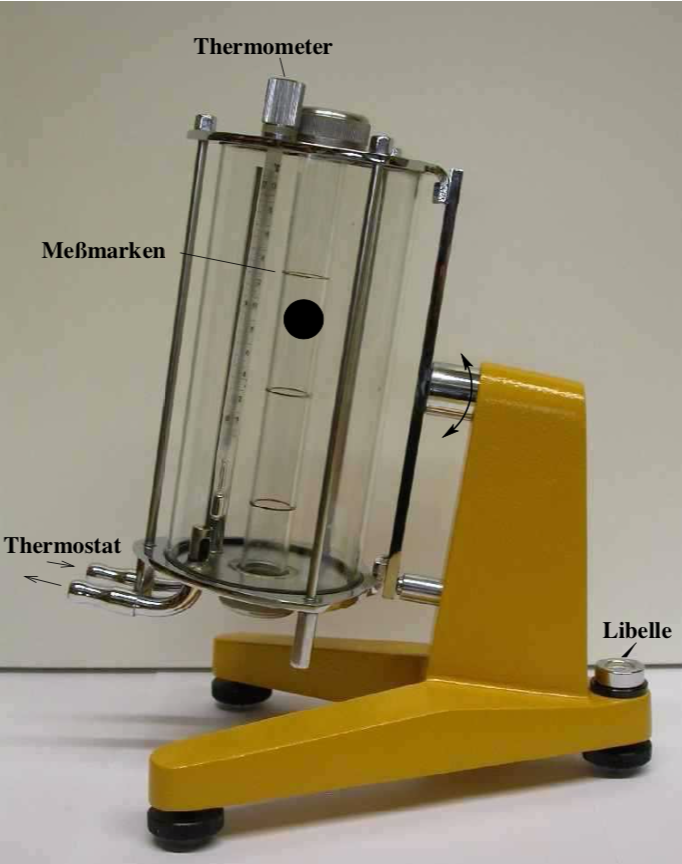
\includegraphics[height=8cm]{Aufbau.png}
    \label{fig:a}
\end{figure}
